\chapter{Task 21: Dynamics on network}
\resp{Andrea Santarossa}

\noindent\textcolor{unipd}{\textit{Epidemic spreading on static networks: SI, SIS, SIR, SEIR in homogeneous and heterogeneous mean-field approximation.}}

Modeling epidemic spreading is a challenging problem due to the intrinsic complexity of contagion processes, which emerge from the interplay between biological mechanisms, human behavior, and social interactions. The difficulty of collecting detailed interaction data, together with ethical and privacy constraints, makes it hard to construct fully realistic models. For this reason, epidemic spreading is commonly studied through compartmental models (see Appendix~\ref{app:comp_models}), where individuals are assigned to discrete epidemiological states such as SI, SIS, SIR, and SEIR, allowing for a simplified but effective description of the dynamics. A natural extension of these models is to consider epidemic spreading on contact networks, where nodes represent individuals and links represent possible transmission pathways. This framework makes it possible to investigate how the structure of interactions affects the spreading dynamics. The aim of this task is to analyze SI, SIS, SIR, and SEIR models on static networks within homogeneous and heterogeneous mean-field approximations, comparing different network topologies and studying how the epidemic (invasion) threshold depends on the model parameters and on network heterogeneity.

\section{Mathematical framework}\label{sec:math}

The spreading of an epidemic on a network can be described as a stochastic dynamical process in which each node represents an individual and each edge represents a potential transmission channel, as discussed in \cite{epidemics}. The state of each node evolves in time according to the infection and recovery mechanisms, which depend on the states of its neighbors. In general, this leads to a high-dimensional stochastic process that is analytically intractable for large systems. For this reason, mean-field approximations are commonly employed to derive a tractable mathematical description of the dynamics.

In the homogeneous mean-field (HMF) approximation, all nodes are assumed to be statistically equivalent, and the network structure is encoded only through the average degree $\langle k \rangle$. Under this assumption, the probability that a node is infected depends only on the global density of infected individuals. For instance, in the case of a generic SIS-like dynamics, the time evolution of the infected density $I(t)$ can be approximated by:
\begin{equation}
\frac{dI}{dt} = \beta \langle k \rangle I(t)\left[1 - I(t)\right] - \mu I(t),
\end{equation}
where $\beta$ is the infection rate and $\mu$ is the recovery rate. This equation captures the competition between infection and recovery processes, assuming that each node interacts with an average number of neighbors.

A key quantity emerging from this description is the epidemic threshold, which determines whether the infection can invade the system or dies out. This threshold can be expressed in terms of a critical infection rate $\beta_c$, defined as:
\begin{equation}
\beta_c = \frac{\mu}{\langle k \rangle}.
\end{equation}
For $\beta < \beta_c$, the infection cannot sustain itself and eventually disappears, while for $\beta > \beta_c$ a finite fraction of the population remains infected in the stationary state.

However, real networks are often heterogeneous, with a broad distribution of node degrees. In this case, the homogeneous approximation fails to capture the role of highly connected nodes. The heterogeneous mean-field approach accounts for this by grouping nodes according to their degree $k$ and introducing degree-dependent densities $I_k(t)$. The evolution equations then become:
\begin{equation}
\frac{dI_k}{dt} = \beta k \left[1 - I_k(t)\right] \Theta(t) - \mu I_k(t),
\end{equation}
where $\Theta(t)$ represents the probability that a randomly chosen neighbor is infected. This quantity depends on the degree distribution and introduces a coupling between different degree classes.

Within this framework, the epidemic threshold is again expressed in terms of a critical infection rate, which now explicitly depends on the heterogeneity of the network:
\begin{equation}
\beta_c = \mu \frac{\langle k \rangle}{\langle k^2 \rangle}.
\end{equation}
This result highlights the crucial role of degree fluctuations: in networks with large variance (such as scale-free networks), the second moment $\langle k^2 \rangle$ can diverge, leading to a vanishing epidemic threshold in the thermodynamic limit. As a consequence, even infections with very small transmission rates can spread and persist in highly heterogeneous networks.


\section{Epidemic dynamics on homogeneous networks}

In this section, we investigate epidemic spreading on a homogeneous network, modeled as an Erdős--Rényi random graph. In this setting, nodes have approximately the same number of connections, and the network can be reasonably described within a homogeneous mean-field approximation.

To validate this assumption, we compare three different descriptions of the dynamics: (i) stochastic simulations on the network, averaged over multiple independent realizations, (ii) the deterministic mean-field ordinary differential equations (ODEs), and (iii) a discrete-time binomial chain approximation \cite{book_epidemics}. The comparison is shown in Fig.~\ref{fig:infected_comparison}, where the temporal evolution of the infected fraction $I(t)$ is reported for different epidemic models.

Further details on the implementation of the models and the binomial chain approximation are provided in Appendix~\ref{app:hom_net}.

\begin{figure}[!htbp]
    \centering
    \makebox[\textwidth][c]{
        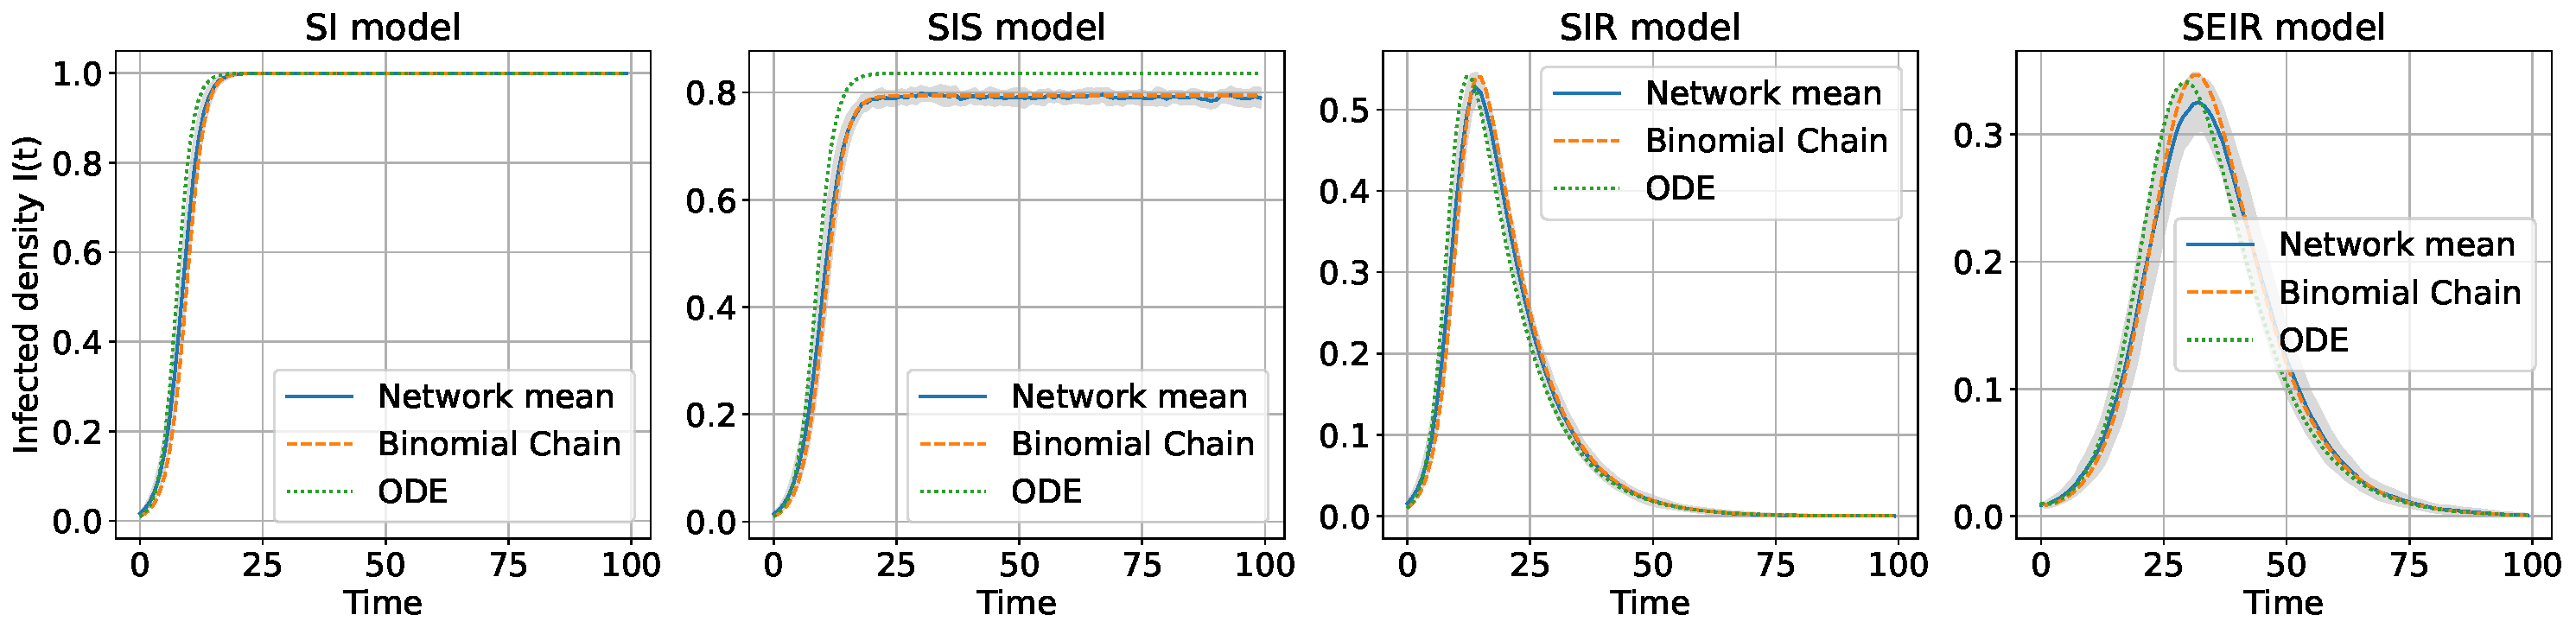
\includegraphics[width=1.2\textwidth]{plots/infected_comparison.pdf}
    }
    \captionsetup{
        width=1.2\textwidth,
        font={footnotesize,stretch=0.9},
        labelfont=bf,
        skip=3pt
    }
    \caption{Comparison of the infected fraction $I(t)$ for different epidemic models (SI, SIS, SIR, SEIR) on a homogeneous Erdős--Rényi network. The network consists of $N = 1000$ nodes with link probability $p = 0.03$ (average degree $k = 30.5$). The simulations are run for $T = 100$ timesteps with infection rate $\beta = 0.02 > \beta_c$ , recovery rate $\mu = 0.1$, and incubation rate $\sigma = 0.2$ (for SEIR). The initial condition is $I_0 = 10$ infected nodes. Results are averaged over $25$ independent runs. The shaded area represents one standard deviation around the mean of the network-based simulations, while dashed and dotted lines correspond respectively to the binomial chain approximation and the deterministic ODE model.}
    \label{fig:infected_comparison}
\end{figure}


\section{Epidemic dynamics on heterogeneous networks}

We extend the analysis to heterogeneous networks by considering three topologies: Erdős--Rényi, Small-World (Watts--Strogatz), and Scale-Free (Barabási--Albert). For each network, epidemic dynamics (SI, SIS, SIR, SEIR) are simulated, and results are averaged over multiple independent runs. We report the mean fraction of infected nodes over time. Figure~\ref{fig:infected_networks} shows the comparison between the three network topologies, while implementation details are reported in Appendix~\ref{app:het_net}.

\begin{figure}[!htbp]
    \centering
    \makebox[\textwidth][c]{
        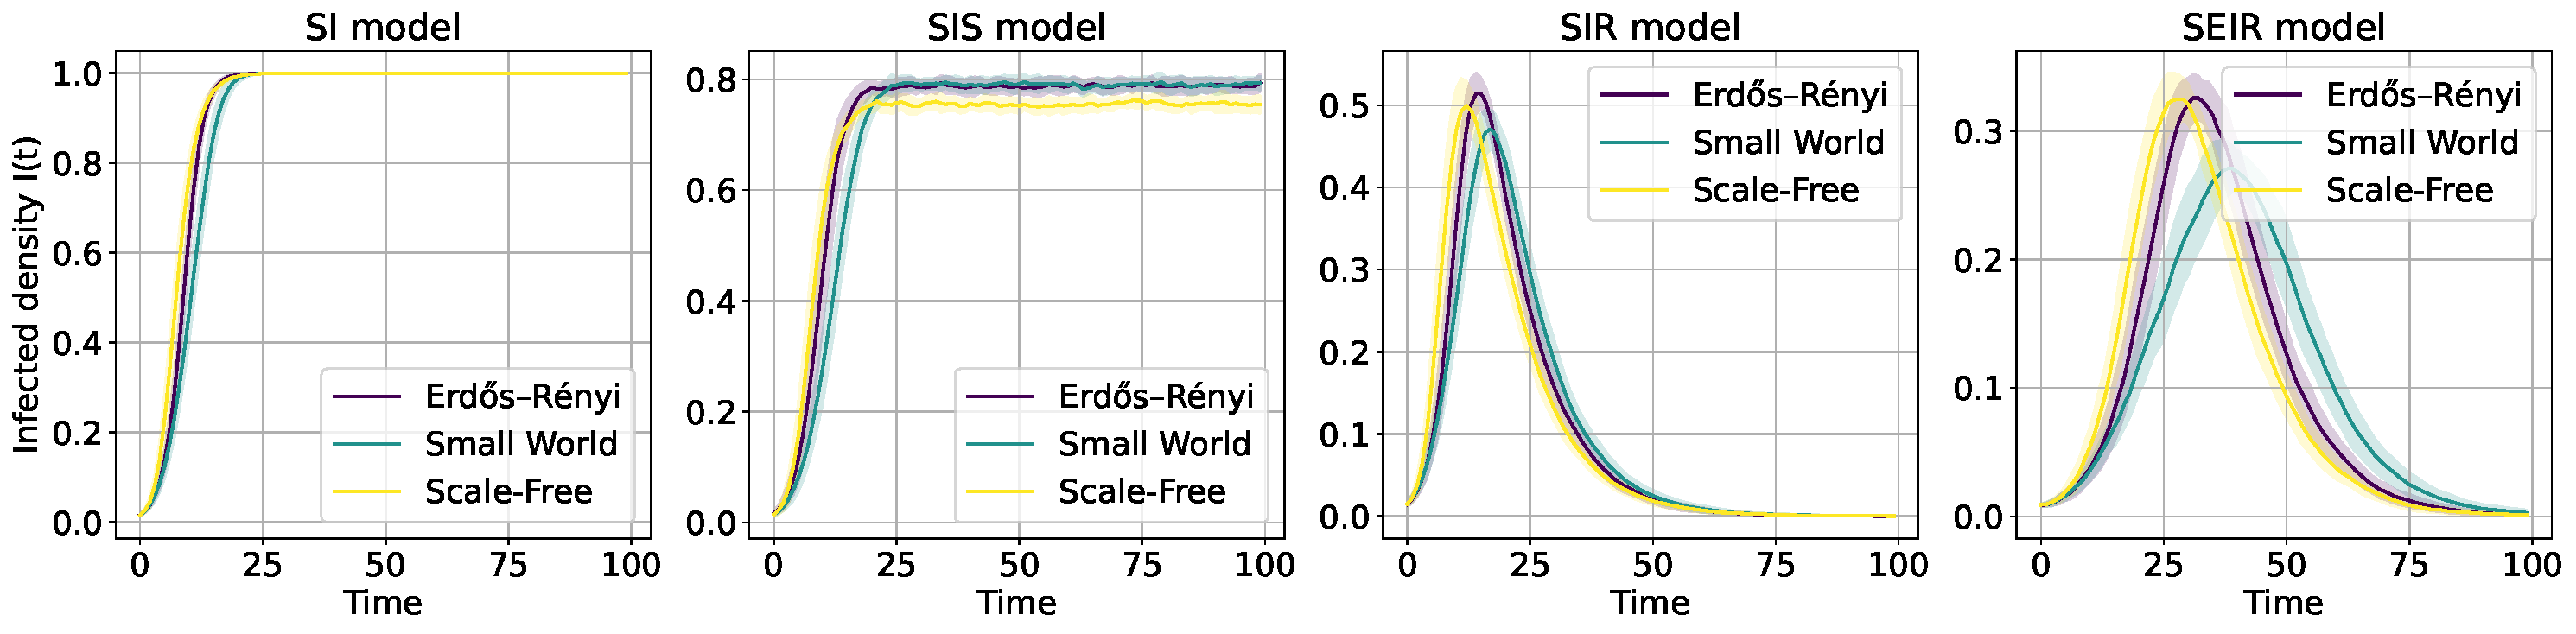
\includegraphics[width=1.2\textwidth]{plots/infected_networks_comparison.pdf}
    }
    \captionsetup{
        width=1.2\textwidth,
        font={footnotesize,stretch=0.9},
        labelfont=bf,
        skip=3pt
    }
    \caption{Comparison of the infected fraction $I(t)$ for different epidemic models (SI, SIS, SIR, SEIR) across networks with different topological properties: Erdős--Rényi (homogeneous), Small-World (Watts--Strogatz), and Scale-Free (Barabási--Albert). Each panel corresponds to a different epidemic model, while curves represent different network topologies. All networks consist of $N = 1000$ nodes. The Erdős--Rényi network has link probability $p = 0.03$, the Small-World network is generated with $k_0 = 30$ and rewiring probability $p = 0.1$, and the Scale-Free network is constructed with $m = 15$. Simulations are run for $T = 100$ timesteps with infection rate $\beta = 0.02$, recovery rate $\mu = 0.1$, and incubation rate $\sigma = 0.2$ (for SEIR). The initial condition is $I_0 = 10$ infected nodes. Results are averaged over $25$ independent runs, and the shaded area represents one standard deviation around the mean.}
    \label{fig:infected_networks}
\end{figure}


\subsection{Epidemic threshold}

To investigate the epidemic threshold, we use the Heterogeneous Mean-Field (HMF) approximation introduced in Section~\ref{sec:math}. For each network, we numerically compute the moments of the degree distribution and estimate the corresponding theoretical epidemic threshold $\beta_c$, reported in Table~\ref{tab:thresholds}.

\begin{table}[h]
\centering
\begin{tabular}{cccc}
\hline
\textbf{Network} & $\mathbf{\langle k \rangle}$ & $\mathbf{\langle k^2 \rangle}$ & $\boldsymbol{\beta_c}$ \\
\hline
Erdős--Rényi    & 4.02 & 20.3 & 0.040 \\
Small-world     & 4.00 & 16.8 & 0.048 \\
Scale-free (BA) & 3.99 & 45.2 & 0.018 \\
\hline
\end{tabular}
\caption{Degree moments and theoretical epidemic threshold $\beta_c$ for different network topologies.}
\label{tab:thresholds}
\end{table}

For each network, we run 400 simulations of the SIR dynamics for different values of $\beta$ and compute the final attack rate, defined as $R_{\infty} = \frac{R(T)}{N},$ averaged over multiple runs, in order to validate the theoretical predictions. The resulting plot is shown in Fig.~\ref{fig:epid_thr}, while the details of the network models used and the corresponding degree distributions are reported in Appendix~\ref{app:epid_thr}.


\begin{figure}[!htbp]
    \centering
    \makebox[\textwidth][c]{
        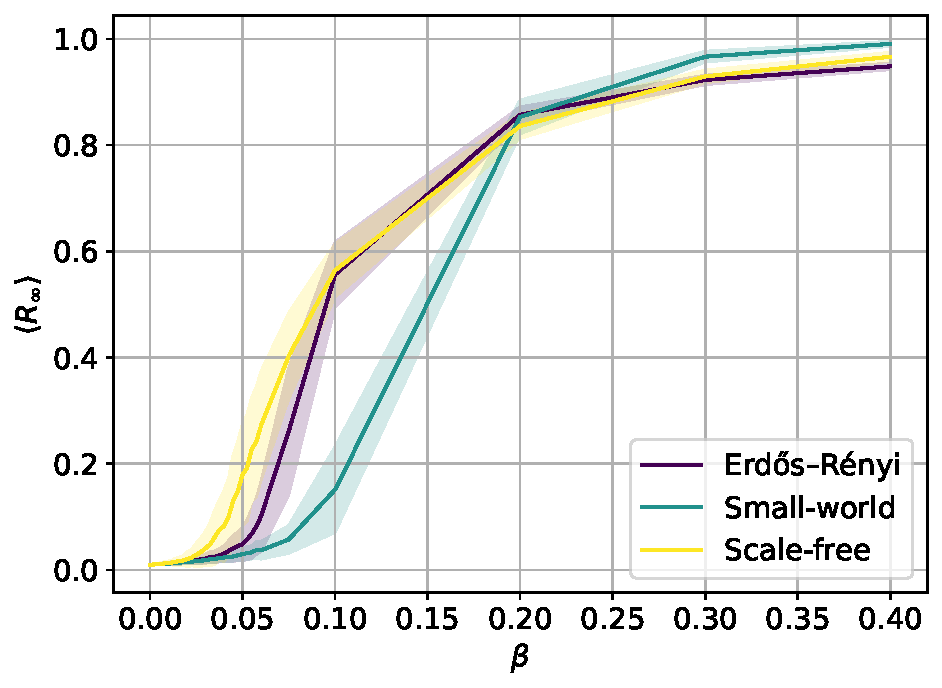
\includegraphics[width=0.75\textwidth]{plots/epidemic_threshold.pdf}
    }
    \captionsetup{
        width=1.2\textwidth,
        font={footnotesize,stretch=0.9},
        labelfont=bf,
        skip=3pt
    }
    \caption{Final attack rate $\langle R_\infty \rangle$ as a function of the infection rate $\beta$ for different network topologies: Erdős--Rényi, small-world, and scale-free (Barabási--Albert). Each point is averaged over $n_{\mathrm{runs}} = 400$ independent SIR simulations with $N=1000$ nodes and recovery rate $\mu = 0.2$, starting from a single infected node. Shaded regions represent the standard deviation.}
    \label{fig:epid_thr}
\end{figure}


\section{Conclusion}

Real-world contact networks are typically heterogeneous and often display scale-free properties. As shown in this report, scale-free networks are significantly more prone to epidemic spreading due to the reduced (or vanishing) epidemic threshold $\beta_c$ induced by large degree fluctuations.

This structural property has important implications for control strategies. In particular, random immunization is suboptimal, while more effective approaches exploit network heterogeneity by targeting highly connected nodes. A representative example is acquaintance immunization, which selects individuals through their neighbors rather than uniformly at random (see Appendix~\ref{app:acquaintance_immunization}), and significantly improves containment efficiency, as shown in the numerical comparison in the Appendix.

\newpage